\documentclass[border=10pt]{standalone}
\usepackage{tikz}
\usetikzlibrary{arrows.meta,positioning,fit,backgrounds,calc,shapes.geometric}

% ---- palette ----
\definecolor{cInk}{RGB}{30,41,59}
\definecolor{cInputF}{RGB}{224,231,255}\definecolor{cInputD}{RGB}{79,70,229}
\definecolor{cP1F}{RGB}{239,246,255}\definecolor{cP1D}{RGB}{59,130,246}
\definecolor{cMgrF}{RGB}{254,243,199}\definecolor{cMgrD}{RGB}{217,119,6}
\definecolor{cSomF}{RGB}{236,253,245}\definecolor{cSomD}{RGB}{13,148,136}
\definecolor{cAgF}{RGB}{255,255,255}\definecolor{cAgD}{RGB}{100,116,139}
\definecolor{cLogF}{RGB}{237,233,254}\definecolor{cLogD}{RGB}{124,58,237}
\definecolor{cQaF}{RGB}{255,237,213}\definecolor{cQaD}{RGB}{234,88,12}
\definecolor{cExF}{RGB}{254,226,226}\definecolor{cExD}{RGB}{220,38,38}
\definecolor{cP2F}{RGB}{236,253,245}\definecolor{cP2D}{RGB}{16,185,129}
\definecolor{cPhyF}{RGB}{209,250,229}\definecolor{cPhyD}{RGB}{5,150,105}
\definecolor{cP3F}{RGB}{250,245,255}\definecolor{cP3D}{RGB}{147,51,234}
\definecolor{cRepF}{RGB}{233,213,255}\definecolor{cRepD}{RGB}{126,34,206}
\definecolor{cRagF}{RGB}{248,250,252}\definecolor{cRagD}{RGB}{71,85,105}
\definecolor{cDomF}{RGB}{241,245,249}\definecolor{cDomD}{RGB}{100,116,139}
\definecolor{cOutF}{RGB}{254,249,195}\definecolor{cOutD}{RGB}{202,138,4}
\definecolor{cAppF}{RGB}{220,252,231}\definecolor{cAppD}{RGB}{22,163,74}
\definecolor{cFeed}{RGB}{220,38,38}

\begin{document}
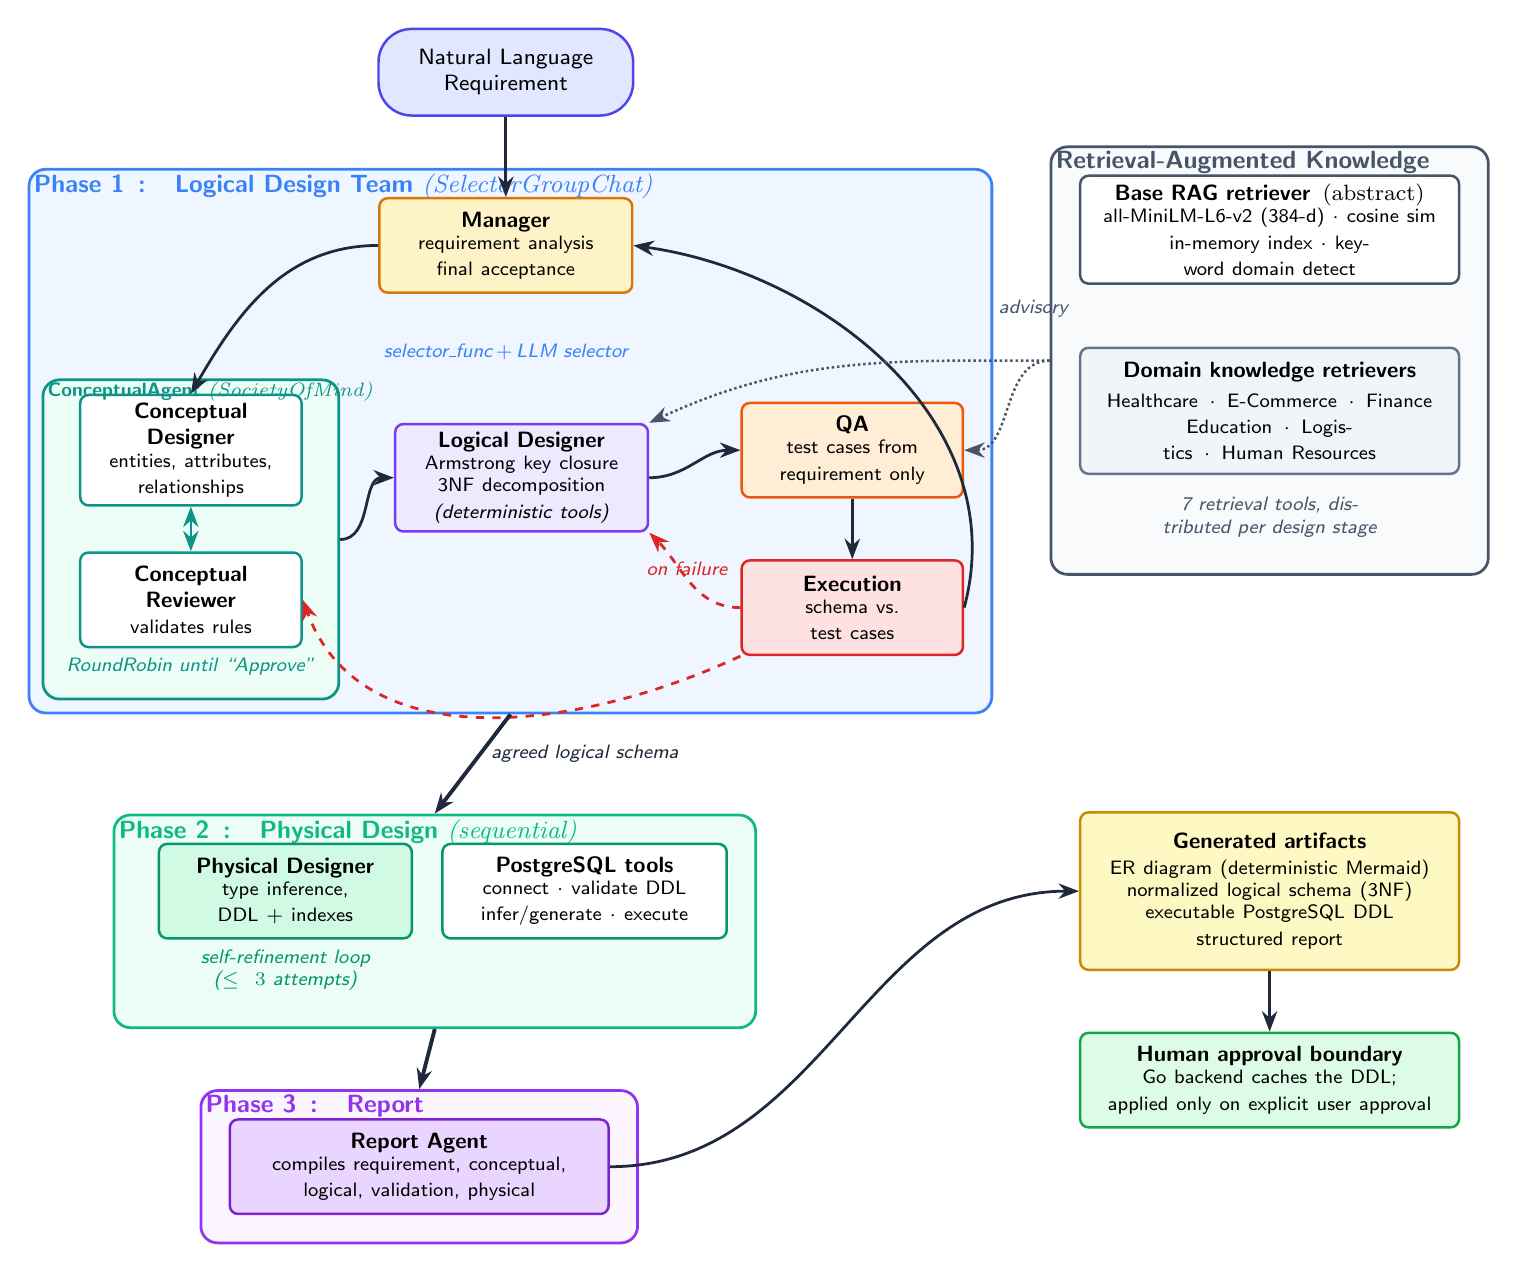
\begin{tikzpicture}[
  font=\sffamily, line width=0.5pt, >={Stealth[length=2.6mm]},
  band/.style={rounded corners=6pt, draw, line width=1pt, inner sep=10pt},
  bandlbl/.style={font=\sffamily\bfseries\small, anchor=north west, inner sep=2pt},
  agent/.style={rounded corners=3pt, draw, line width=0.9pt, align=center,
    text width=26mm, minimum height=12mm, font=\sffamily\footnotesize, inner sep=3pt},
  wide/.style={agent, text width=46mm},
  io/.style={rounded corners=12pt, draw, line width=0.9pt, align=center,
    fill=cInputF, draw=cInputD, text width=30mm, minimum height=11mm, font=\sffamily\footnotesize},
  note/.style={font=\sffamily\scriptsize\itshape, text=cInk, align=center},
  flow/.style={->, line width=1pt, draw=cInk},
  bigflow/.style={->, line width=1.4pt, draw=cInk},
  feed/.style={->, line width=1pt, draw=cFeed, dashed},
  rag/.style={->, line width=0.9pt, draw=cRagD, densely dotted},
]

% =================== NODES (absolute coords, cm) ===================
% ---- input ----
\node[io] (req) at (5.7,1.4) {Natural Language\\Requirement};

% ---- Phase 1 agents ----
\node[agent, fill=cMgrF, draw=cMgrD, text width=30mm] (mgr) at (5.7,-0.8)
  {\textbf{Manager}\\\scriptsize requirement analysis\\\scriptsize final acceptance};
\node[note, text=cP1D] (selnote) at (5.7,-2.15) {selector\_func\,$+$\,LLM selector};

% society of mind
\node[agent, fill=cAgF, draw=cSomD] (cdes) at (1.7,-3.4)
  {\textbf{Conceptual}\\\textbf{Designer}\\\scriptsize entities, attributes,\\\scriptsize relationships};
\node[agent, fill=cAgF, draw=cSomD] (crev) at (1.7,-5.3)
  {\textbf{Conceptual}\\\textbf{Reviewer}\\\scriptsize validates rules};
\node[note, text=cSomD] (looplbl) at (1.7,-6.15) {RoundRobin until ``Approve''};

\node[agent, fill=cLogF, draw=cLogD, text width=30mm] (log) at (5.9,-3.75)
  {\textbf{Logical Designer}\\\scriptsize Armstrong key closure\\\scriptsize 3NF decomposition\\\scriptsize \textit{(deterministic tools)}};

\node[agent, fill=cQaF, draw=cQaD] (qa) at (10.1,-3.4)
  {\textbf{QA}\\\scriptsize test cases from\\\scriptsize requirement only};
\node[agent, fill=cExF, draw=cExD] (exe) at (10.1,-5.4)
  {\textbf{Execution}\\\scriptsize schema vs.\\\scriptsize test cases};

% ---- Phase 2 agents ----
\node[agent, fill=cPhyF, draw=cPhyD, text width=30mm] (phy) at (2.9,-9.0)
  {\textbf{Physical Designer}\\\scriptsize type inference,\\\scriptsize DDL $+$ indexes};
\node[agent, fill=cAgF, draw=cPhyD, text width=34mm] (pgtools) at (6.7,-9.0)
  {\textbf{PostgreSQL tools}\\\scriptsize connect $\cdot$ validate DDL\\\scriptsize infer/generate $\cdot$ execute};
\node[note, text=cPhyD, text width=34mm] (reflbl) at (2.9,-10.0) {self-refinement loop ($\leq 3$ attempts)};

% ---- Phase 3 agent ----
\node[agent, fill=cRepF, draw=cRepD, text width=46mm] (rep) at (4.6,-12.5)
  {\textbf{Report Agent}\\\scriptsize compiles requirement, conceptual,\\\scriptsize logical, validation, physical};

% ---- RAG panel (right) ----
\node[wide, fill=cAgF, draw=cRagD, minimum height=10mm] (baserag) at (15.4,-0.6)
  {\textbf{Base RAG retriever}\, \textnormal{(abstract)}\\\scriptsize all-MiniLM-L6-v2 (384-d) $\cdot$ cosine sim\\\scriptsize in-memory index $\cdot$ keyword domain detect};
\node[wide, fill=cDomF, draw=cDomD, minimum height=16mm] (domains) at (15.4,-2.9)
  {\textbf{Domain knowledge retrievers}\\[1mm]
   \scriptsize Healthcare\, $\cdot$\, E-Commerce\, $\cdot$\, Finance\\\scriptsize Education\, $\cdot$\, Logistics\, $\cdot$\, Human Resources};
\node[note, text=cRagD, text width=46mm] (ragtoolslbl) at (15.4,-4.25)
  {7 retrieval tools, distributed per design stage};

% ---- Outputs + approval (right, lower) ----
\node[wide, fill=cOutF, draw=cOutD, minimum height=20mm] (out) at (15.4,-9.0)
  {\textbf{Generated artifacts}\\[0.5mm]
   \scriptsize ER diagram (deterministic Mermaid)\\\scriptsize normalized logical schema (3NF)\\\scriptsize executable PostgreSQL DDL\\\scriptsize structured report};
\node[wide, fill=cAppF, draw=cAppD, minimum height=12mm] (approve) at (15.4,-11.4)
  {\textbf{Human approval boundary}\\\scriptsize Go backend caches the DDL;\\\scriptsize applied only on explicit user approval};

% =================== CONTAINERS ===================
\begin{scope}[on background layer]
  \node[band, fill=cP1F, draw=cP1D,
        fit=(mgr)(selnote)(cdes)(crev)(looplbl)(log)(qa)(exe)] (p1) {};
  \node[band, fill=cP2F, draw=cP2D, fit=(phy)(pgtools)(reflbl)] (p2) {};
  \node[band, fill=cP3F, draw=cP3D, fit=(rep)] (p3) {};
  \node[band, fill=cRagF, draw=cRagD, fit=(baserag)(domains)(ragtoolslbl)] (ragbox) {};
\end{scope}
% som band drawn after p1 so it sits on top
\begin{scope}[on background layer]
  \node[band, fill=cSomF, draw=cSomD, inner sep=5pt, fit=(cdes)(crev)(looplbl)] (som) {};
\end{scope}

\node[bandlbl, text=cP1D] at (p1.north west) {Phase 1\, : \, Logical Design Team \textnormal{\itshape (SelectorGroupChat)}};
\node[bandlbl, text=cSomD, yshift=1pt] at (som.north west) {\scriptsize ConceptualAgent \textnormal{\itshape (SocietyOfMind)}};
\node[bandlbl, text=cP2D] at (p2.north west) {Phase 2\, : \, Physical Design \textnormal{\itshape (sequential)}};
\node[bandlbl, text=cP3D] at (p3.north west) {Phase 3\, : \, Report};
\node[bandlbl, text=cRagD] at (ragbox.north west) {Retrieval-Augmented Knowledge};

% =================== ARROWS ===================
% main path
\draw[flow] (req) -- (mgr);
\draw[flow] (mgr.west) to[out=180,in=60] (cdes.north);
\draw[<->, line width=0.9pt, draw=cSomD] (cdes.south) -- (crev.north);
\draw[flow] (som.east) to[out=0,in=180] (log.west);
\draw[flow] (log.east) to[out=0,in=180] (qa.west);
\draw[flow] (qa.south) -- (exe.north);
\draw[flow] (exe.east) to[out=75,in=-8] (mgr.east);

% feedback (validation failures routed back, kept inside Phase 1)
\draw[feed] (exe.west) to[out=180,in=-45] (log.south east);
\draw[feed] (exe.south west) to[out=205,in=-70] (crev.east);
\node[note, text=cFeed] at (8.0,-4.9) {on failure};

% phase transitions
\draw[bigflow] (p1.south) -- node[note, right, pos=0.4]{agreed logical schema} (p2.north);
\draw[bigflow] (p2.south) -- (p3.north);

% report -> artifacts -> approval
\draw[flow] (rep.east) to[out=0,in=180] (out.west);
\draw[flow] (out.south) -- (approve.north);

% RAG advisory (dotted)
\draw[rag] (ragbox.west) to[out=180,in=0] (qa.east);
\draw[rag] (ragbox.west) to[out=180,in=25] (log.north east);
\node[note, text=cRagD] at (12.4,-1.6) {advisory};

\end{tikzpicture}
\end{document}
